\PassOptionsToPackage{top=3cm,left=3cm,right=3cm,bottom=3cm}{geometry}
\documentclass[fleqn,11pt]{wlscirep_supp}

\usepackage[]{minitoc}
\mtcsetdepth{secttoc}{3}
\setcounter{secnumdepth}{2}
\setcounter{tocdepth}{2}
\mtcsettitle{secttoc}{}


\usepackage[utf8]{inputenc}
\usepackage[T1]{fontenc}
\usepackage[english]{babel}
%\usepackage[top=3cm,left=3cm,right=3cm,bottom=3cm]{geometry}% by courtesy of Mico
\usepackage{lmodern}
\usepackage{bbm}
\usepackage{graphicx}
\usepackage{epstopdf}
\usepackage{colortbl}
\usepackage{siunitx}
\sisetup{
  detect-all,
  detect-weight=true,
  detect-family=true,
  mode=text,
%   detect-inline-family=math,
  group-separator={,},
%   group-minimum-digits={3}			
}
\usepackage{rotating}
\usepackage{tabularx}
\usepackage{tabu}
\usepackage{authblk}
\usepackage{mathtools}
\usepackage{overpic}
\usepackage{url}
\usepackage{tikz}
\usetikzlibrary{positioning}
\usetikzlibrary{arrows}
\usetikzlibrary{fit}
\usepackage{multirow}
\usepackage{float}
\usepackage[normalem]{ulem}
\usepackage{bm}
\usepackage{enumerate}
\usepackage[absolute,overlay%,showboxes
                        ]{textpos}
% \usepackage{caption}
\usepackage[font=small,labelfont=bf,justification=justified]{caption}
\usepackage{subcaption}
\usepackage{xspace}
\usepackage[colorinlistoftodos]{todonotes}
\usepackage{placeins}
\usepackage{makecell, booktabs}
\usepackage{eqparbox}
\usepackage{rotating}
\usepackage{graphicx}
\usepackage{xspace}
\usepackage{setspace}
%\usepackage{comment}
\usepackage[resetlabels,labeled]{multibib}
\newcites{Supp}{References}
\usepackage[sort&compress]{cleveref}
\Crefname{appendix}{Supplement}{Supplements}

%\usepackage{mathabx}

% Table formatting packages
\usepackage{dcolumn} % align decimal points in tables
\newcolumntype{d}[1]{D{.}{.}{#1}}
\usepackage{booktabs} 
\usepackage[flushleft]{threeparttable}
\usepackage{siunitx} % align on decimal point in tables
\usepackage{lineno}
\usepackage{etoolbox}

\usepackage{lscape}
\usepackage{longtable}
\usepackage{arydshln}

% math
\usepackage{amsmath,amsfonts,amssymb}
% additional math symbols
\DeclareFontFamily{U}{mathb}{}
\DeclareFontShape{U}{mathb}{m}{n}{
  <-5.5> mathb5
  <5.5-6.5> mathb6
  <6.5-7.5> mathb7
  <7.5-8.5> mathb8
  <8.5-9.5> mathb9
  <9.5-11.5> mathb10
  <11.5-> mathb12
}{}
\DeclareSymbolFont{mathb}{U}{mathb}{m}{n}
\DeclareMathSymbol{\ulsh}{3}{mathb}{"E8}
\DeclareMathSymbol{\ursh}{3}{mathb}{"E9}
\DeclareMathSymbol{\dlsh}{3}{mathb}{"EA}
\DeclareMathSymbol{\drsh}{3}{mathb}{"EB}

%% Patch 'normal' math environments:
\newcommand*\linenomathpatch[1]{%
  \cspreto{#1}{\linenomath}%
  \cspreto{#1*}{\linenomath}%
  \csappto{end#1}{\endlinenomath}%
  \csappto{end#1*}{\endlinenomath}%
}

\linenomathpatch{equation}
\linenomathpatch{gather}
\linenomathpatch{multline}
\linenomathpatch{align}
\linenomathpatch{alignat}
\linenomathpatch{flalign}

\linenumbers

% PLOS formatting
\makeatletter %only needed in preamble
\renewcommand\Large{\@setfontsize\Large{18pt}{18}}
\renewcommand\large{\@setfontsize\large{16pt}{18}}
\makeatother

\addto\captionsenglish{\renewcommand{\figurename}{Figure}}

% \usepackage{xstring}
% \usepackage{etoolbox}
% \usepackage{caption}

% \captionsetup{labelfont=bf,tableposition=top}

% \makeatletter
% \newcommand\formatlabel[1]{%
%     \noexpandarg
%     \IfSubStr{#1}{.}{%
%       \StrBefore{#1}{.}[\firstcaption]%
%       \StrBehind{#1}{.}[\secondcaption]%
%       \textbf{\firstcaption.} \secondcaption}{%
%       #1}%
%       }


% \patchcmd{\@caption}{#3}{\formatlabel{#3}}
% \makeatother

\renewcommand*{\Affilfont}{\normalsize\normalfont}
\renewcommand*{\Authfont}{\normalfont}


% referencing of unnumbered materials and methods
\newcounter{methods}
\renewcommand{\themethods}{Materials and methods}

% Track changes
%\usepackage[markup=underlined]{changes}
\makeatletter
\@namedef{Changes@AuthorColor}{magenta}
\colorlet{Changes@Color}{magenta}
\makeatother


%=====================================================================% Declare

\DeclareSIUnit\eur{\officialeuro}
\DeclareSIUnit\M{M}
\DeclareSIUnit\k{k}

% Widebar symbol
% \DeclareFontFamily{U}{mathx}{\hyphenchar\font45}
% \DeclareFontShape{U}{mathx}{m}{n}{<-> mathx10}{}
% \DeclareSymbolFont{mathx}{U}{mathx}{m}{n}
% \DeclareMathAccent{\widebar}{0}{mathx}{"73}

%=====================================================================% New commands (Macros)

% def
\def\sym#1{\ifmmode^{#1}\else\(^{#1}\)\fi}
\definecolor{darkgreen}{rgb}{0.0, 0.5, 0.0}

% new command
\newcommand{\smallsim}{\smallsym{\mathrel}{\sim}}
\newcommand{\specialcell}[2][c]{%
  \begin{tabular}[#1]{@{}l@{}}#2\end{tabular}}
\newcommand{\specialcellc}[2][c]{%
  \begin{tabular}[#1]{@{}c@{}}#2\end{tabular}}
\newcommand\ie{i.\,e.\xspace}
\newcommand\eg{e.\,g.\xspace}
\newcommand{\dd}[1][]{\mathrm{d}#1}
\newcommand{\BK}[1]{{\color{orange}{BK: #1}}}
\newcommand{\figletter}[1]{{{\fontfamily{\sfdefault}\selectfont \textbf{#1}}}}
\newcommand\TODO[1]{{\color{red}#1}}  
\newcommand{\FIX}[1]{{\color{darkgreen}#1}}  

% renewcommand
\renewcommand\theadfont{\bfseries}
\renewcommand\theadalign{lc}
\renewcommand\cellalign{tl}

\makeatletter

\newbox\@abstract%
\def\abstitle{\textbf{Abstract}}%
\renewenvironment{abstract}{
  \global\setbox\@abstract\vbox\bgroup%
   \noindent
}{%
   \egroup%
}%

\renewcommand*{\Affilfont}{\normalsize\normalfont}
\renewcommand*{\Authfont}{\normalfont}

\addto\captionsenglish{% Replace "english" with the language you use
  \renewcommand{\contentsname}{List of Texts}
}

\def\@maketitle{%
  \newpage
    {\raggedright\fontsize{18pt}{20pt}\selectfont \@title \par}%
    \vskip 0.5em%
    {\large
      \lineskip .5em%
      \begin{tabular}[t]{l}%
        \raggedright \normalsize\mdseries{\@author} %
      \end{tabular}\par}%
      \vskip 1em
%      \raggedright\Large\abstitle\par
%      \vskip 1em
%    {\unvbox\@abstract\par}%
    \par
  \vskip 0.5em
}
  
\makeatother


\renewcommand{\thesection}{Text \arabic{section}}
\usepackage{titlesec}
%\titleformat{\section}{\normalfont\Large\bfseries}{Text \thesection.~#1}{1em}{}
\renewcommand{\thefigure}{S\arabic{figure}}
\renewcommand{\thetable}{S\arabic{table}}

\begin{document}
\doublespacing
\nolinenumbers

\title{\LARGE\singlespacing{\textbf{Supplementary Material} \\ \medskip
Spatiotemporal modeling of \emph{Mycobacterium tuberculosis} transmission risk in a South African primary care clinic using environmental, clinical, and patient movement data}}

% author list
\author[1]{Nicolas Banholzer}
\author[2]{Keren Middelkoop}
\author[2]{Juane Leukes}
\author[3]{Ernest Weingartner}
\author[1]{Remo Schmutz}
\author[1]{Kathrin Zürcher}
\author[1]{Matthias Egger}
\author[2]{Robin Wood}
\author[1*]{Lukas Fenner}

\affil[1]{Institute of Social and Preventive Medicine, University of Bern, Bern, Switzerland}
\affil[2]{Desmond Tutu HIV Centre, Department of Medicine, University of Cape Town, Cape Town, South Africa}
\affil[3]{Institute for Sensors and Electronics, University of Applied Sciences and Arts Northwestern Switzerland, Windisch, Switzerland}

\affil[*]{Corresponding author: lukas.fenner@ispm.unibe.ch }

%\begin{abstract}\normalfont
%The supplementary material contains (1)~the detailed method, (2)~the simulation-based study, (3)~further descriptives, and (4)~the results from the sensitivity analysis.
%\end{abstract}

\flushbottom
\maketitle
\thispagestyle{empty}

%\newpage

\sloppy
\raggedbottom

\newpage

\appendix

\tableofcontents

\listoffigures

\listoftables

%\listoffigures
%\listoftables

\newpage

\section{Processing of tracking data}\label{sec:setting-and-data}

Tracking data required processing before it could be fully used for modeling. The reason is that there were considerably more tracking IDs than what would be expected from the number of registered patients in the clinical database. Visitors of the clinic most likely contributed multiple tracks for several reasons: 
\begin{itemize}
    \item A person moved outside the range of the video sensors and then re-entered. 
    \item An individual may temporarily not have been recognized as a person by the tracking software because the person bowed downwards.
    \item A person may have been temporarily hidden behind another person.
    \item Moving objects such as opening doors may have been recognized as a person, introducing noise.
\end{itemize}
We proceeded in two steps to link back together tracking IDs that most likely belonged to the same person. In the first step, we filtered noise (\ie IDs of less than 10\,s and a total moving distance of less than 2\,m), and then automatically matched the remaining tracks that were less than 10\,s and 3\,m apart while moving or less than 60\,s and 0.5\,m apart while sitting. In the second step, we build on the automatically matched tracking data and, through manual inspection, linked tracks that were further apart but still most likely of the same person. To facilitate the manual linkage, we developed a Shiny application and a matching manual (\url{https://github.com/nbanho/clinic-transmission/wiki/Matching-Manual}) that assisted the students who were performing this linkage. 

The Shiny app is shown in \Cref{fig:shiny-app}. In the center panel, a floor plan of the clinic is shown in (x,y)-space. Different areas of the clinic are delineated by colors, \eg seating areas are marked in purple and exit areas are marked in blue. Tracks are shown as lines with an open circle indicating the start and a crossed circle indicating the end of a track. The currently selected track is shown in black, possible links are shown in colors (here only one possible link shown in red), and alternatives to the selected possible link are shown in light grey. 

Below the floor plan is a table showing descriptive information about the possible links in relation to the currently selected track: (1)~the patient ID (Pid) of the selected track and observation ID (Oid) of the possible link, (2)~the height difference between the end of the Pid and end of the Oid track, (3)~ the standing height (\ie maximum height of a track) difference, (4)~the duration of the possible link, (5)~the time difference, and (6)~the distance between the end of the selected track and the start of the selected possible link. Possible links are sorted in ascending order by the time difference. 

In the left panel of \Cref{fig:shiny-app}, the Shiny app first shows descriptive information: the loaded file, the date of the tracking data, the initial number of IDs before any manual linkages, the current number of IDs after considering manual linkages, and the current number of made linkages. It then shows the current Pid with shortcuts to move to the next or previous Pid, or the next or previous Pid at the entrance. Linkages can be done either forward or backward in time. The duration of the current Pid (time in the clinic) is shown together with the number of linked raw tracks of which the current Pid consists. The sliding bars allow filtering of possible links according to difference in time, distance, or height, with pre-set filters above to quickly switch between common thresholds. The first dropdown menu selects the Oid for which alternative matches should be shown in the floor plan. The idea of this feature is to prevent false linkages when there are more plausible alternatives. A linkage is made by selecting the Oid in the "Link with IDs" dropdown menu and clicking "Link IDs". After that, the app updates the floor plan, table, and information in the panel. If an erroneous link was made, it can be revoked by clicking "Unlink last ID" if the last link in time should be revoked or by clicking "Unlink first ID" if the first link in time should be revoked. If no further linkages could be made, the track can be finished by entering a label (see below). The manually linked dataset is automatically saved to the file shown in the bottom of the left panel.

We created labels to denote finished tracks: 
\begin{itemize}
    \item \textbf{Clean}: A clean track throughout the clinic with known entrance and exit.
    \item \textbf{Staff}: IDs with moving in- and out of the staff room.
    \item \textbf{Noise}: A short track ($\leq$1\,min) without entrance or exit.
    \item \textbf{Lost enter}: A long track (>1\,min) without entrance.
    \item \textbf{Lost exit}: A long track (>1\,min) without exit.
    \item \textbf{Lost both}: A long track (>1\,min) without entrance and without exit.
\end{itemize}

\begin{figure}[!htpb]
    \centering
    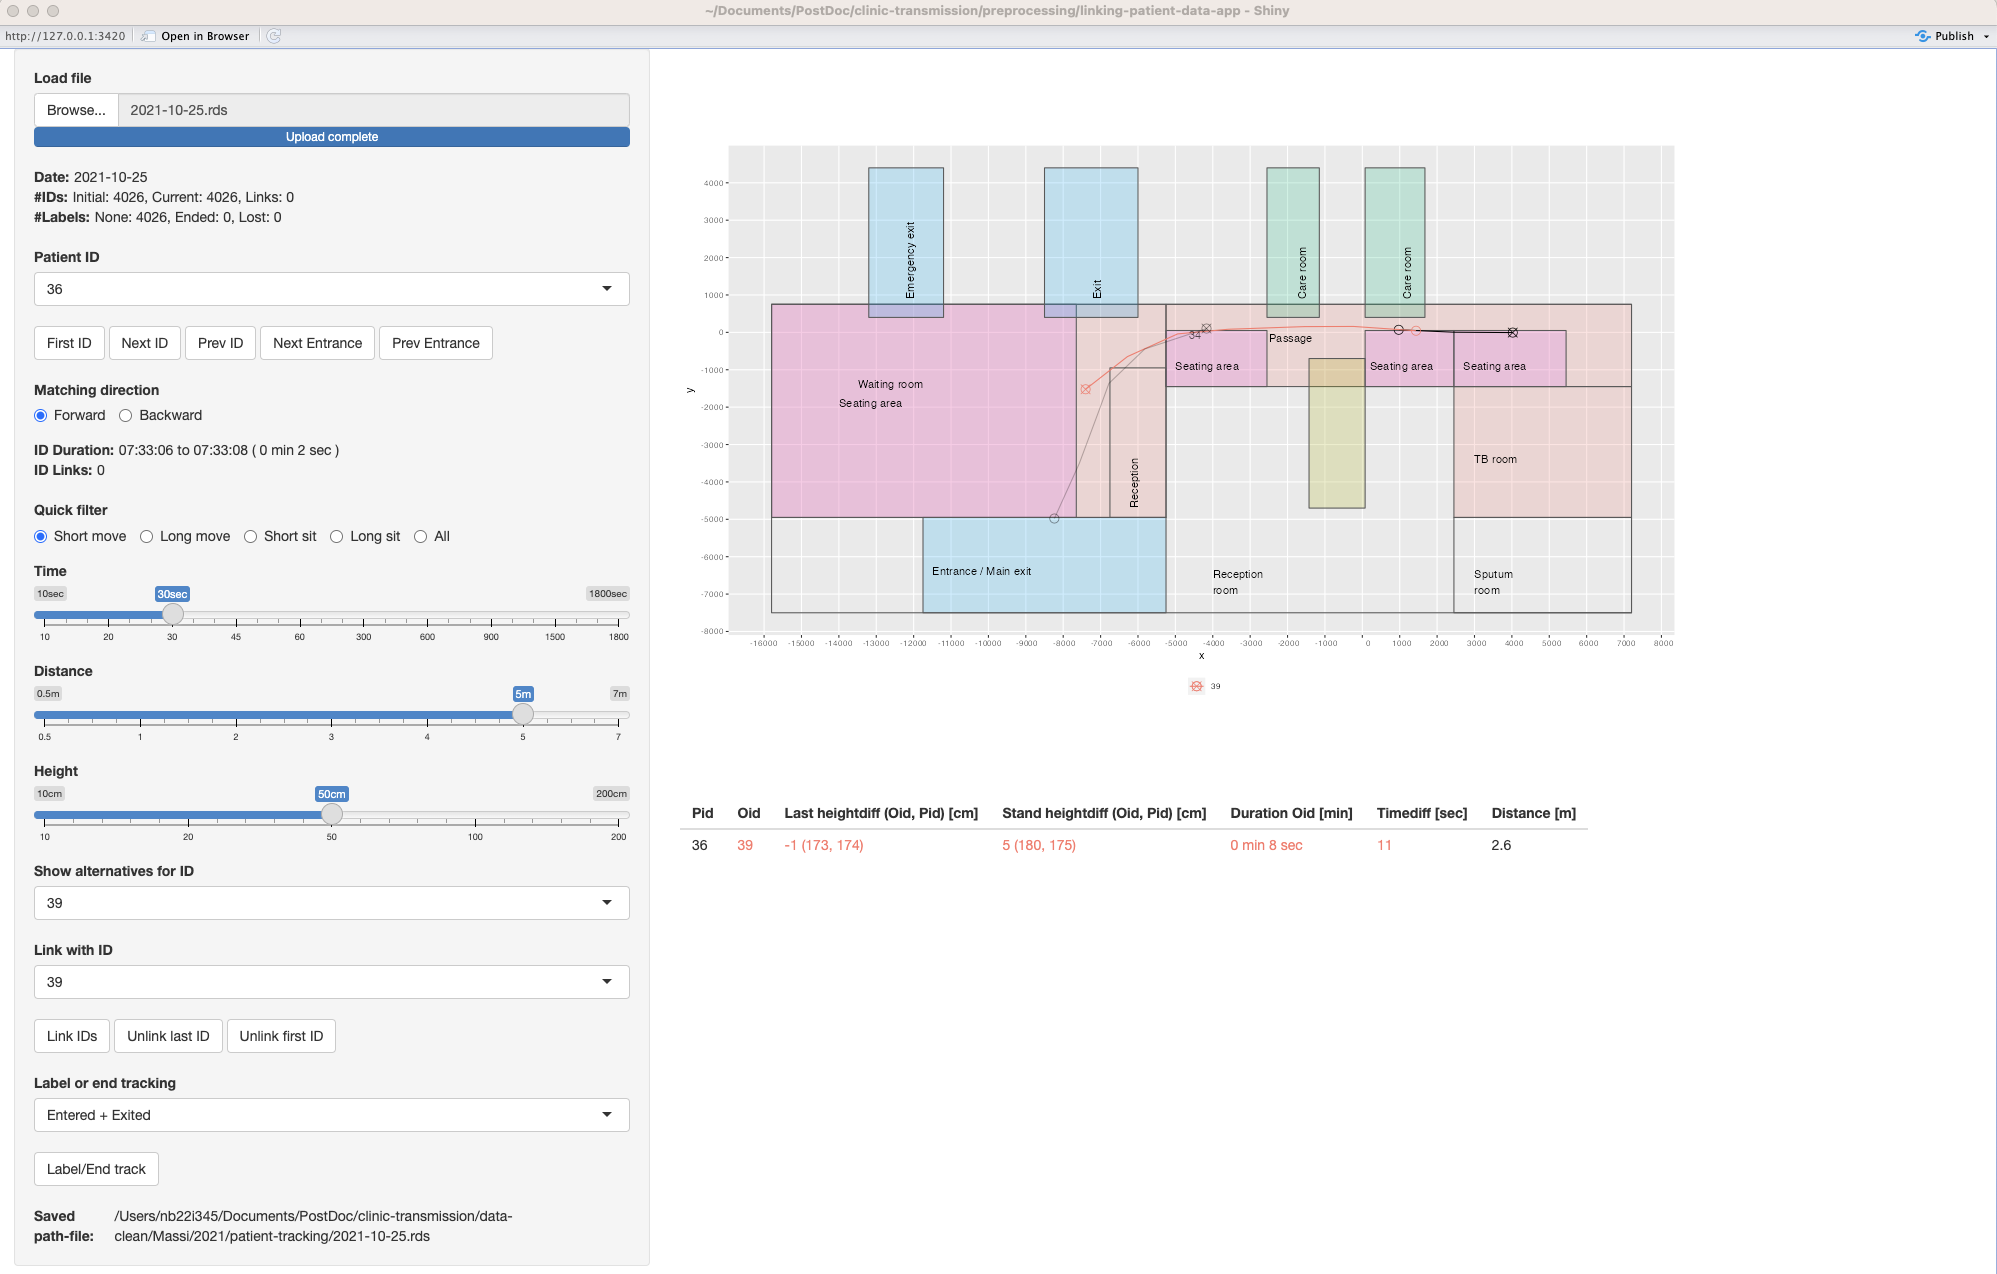
\includegraphics[width=\linewidth]{doc/paper/shiny-tool-screenshot.png}
    \caption{Screenshot of the Shiny app used for manual linking tracking IDs that probably belong together.}
    \label{fig:shiny-app}
\end{figure}

After manual processing of the tracking data, we arrived at 3,319 tracks. We then filtered noise and short tracks <5\,min to obtain 1,563 used for analysis: 209 (13\%) "Clean", 125 (8\%) "Staff", 213 (14\%) "Lost enter", 246 (16\%) "Lost exit", and 770 (49\%) "Lost both". A sample of our tracks used for analysis, excluding staff, are shown in \Cref{fig:tracking-examples}.

\begin{figure}[!htpb]
    \centering
    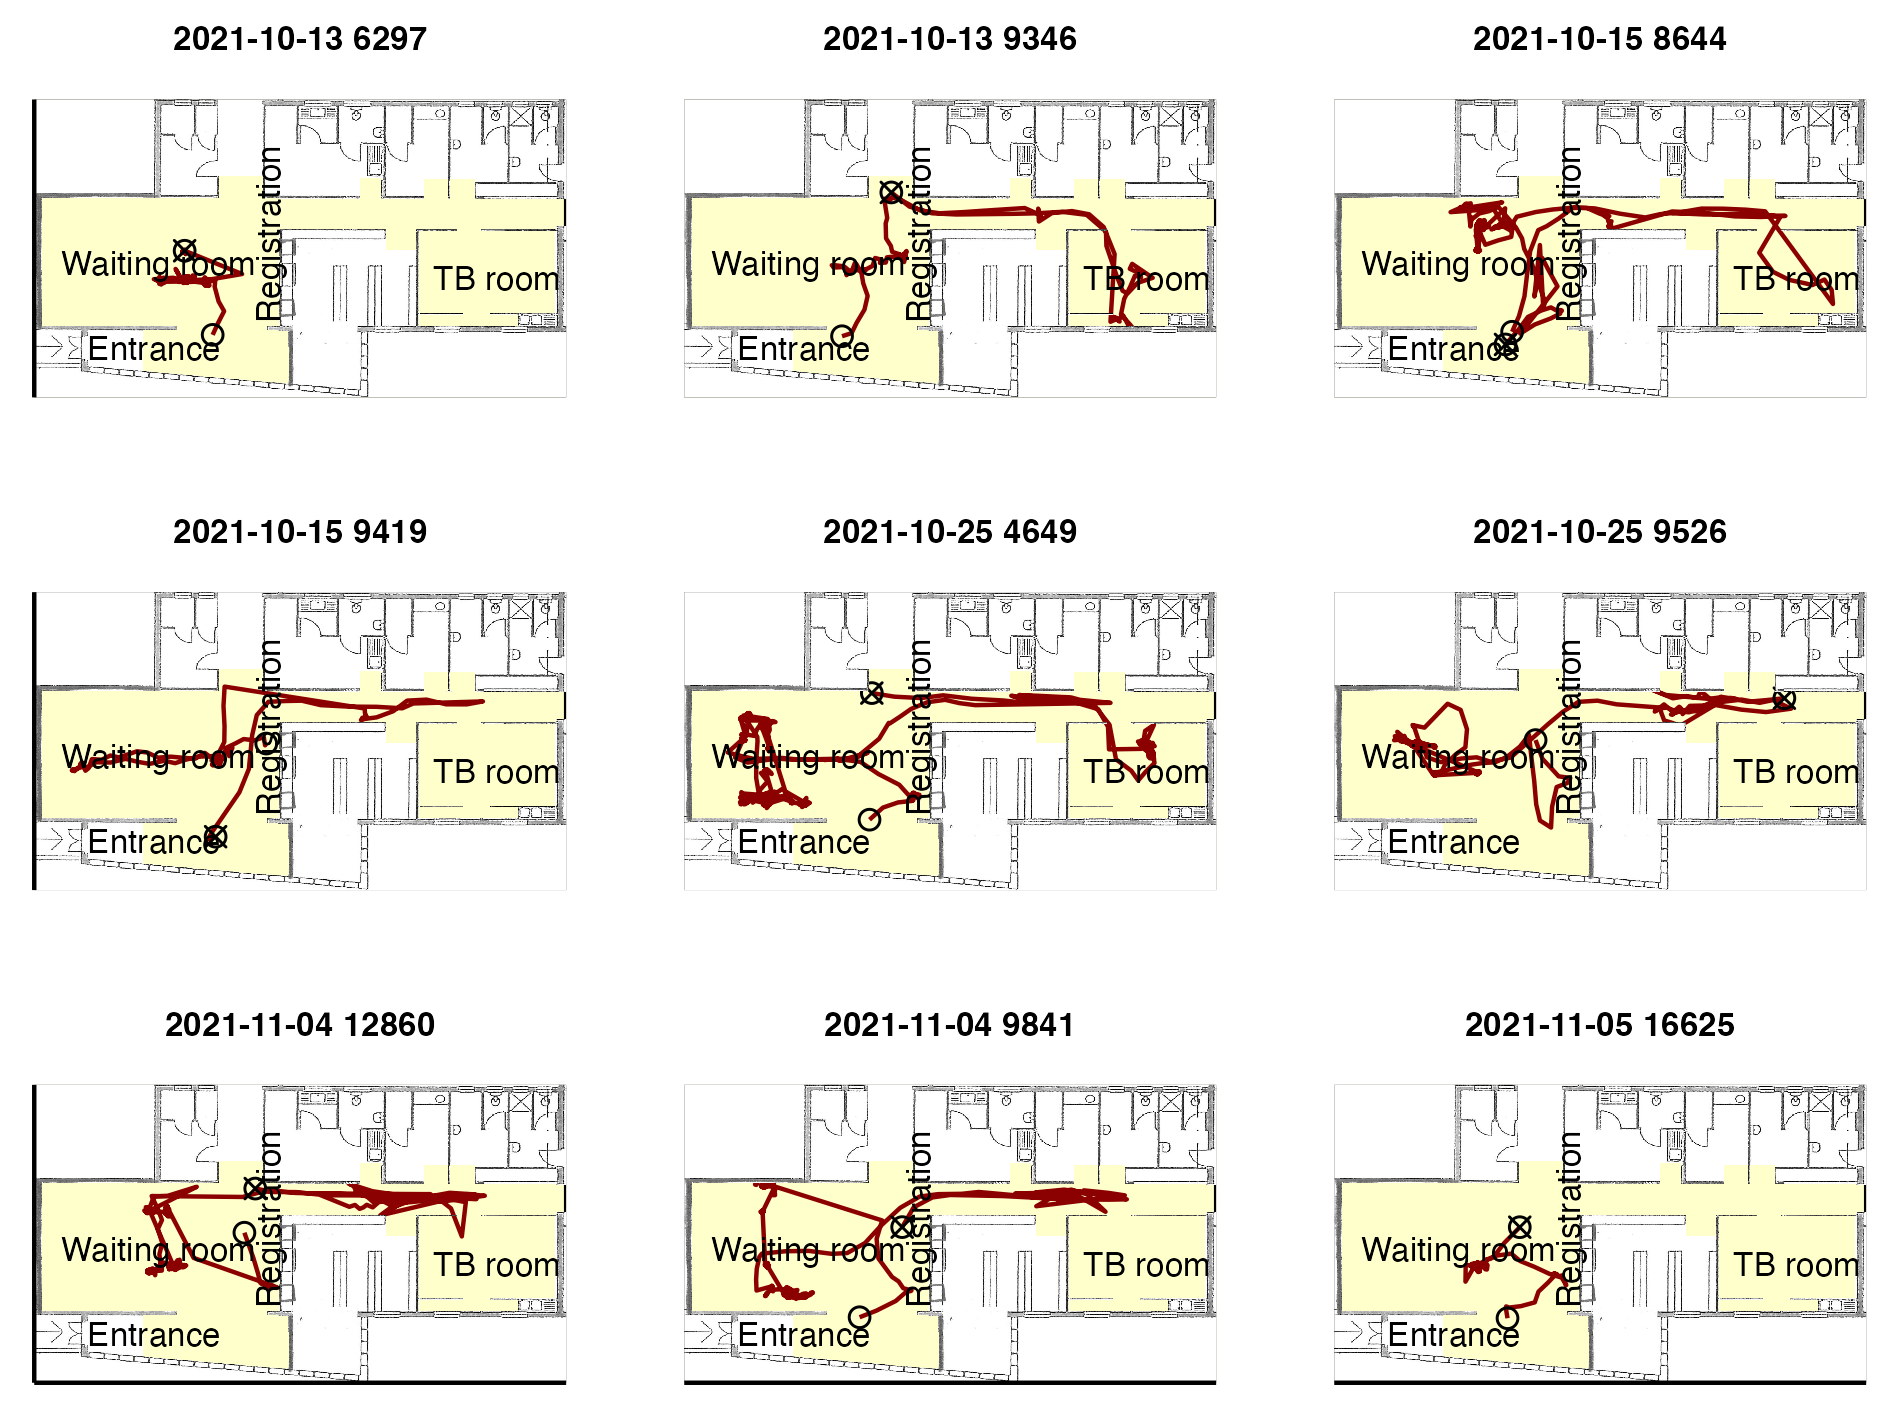
\includegraphics{results/data/example-patient-tracks.png}
    \caption{Sample tracks from our video sensors of this study.}
    \label{fig:tracking-examples}
\end{figure}

\clearpage

\section{Spatiotemporal model}\label{sec:spattemp-model}

\subsection{The Wells-Riley modeling framework}

We build upon the Wells-Riley model\cite{Riley1978AJE}, which is an established epidemiological model to estimate the risk of infection. The model estimates the risk (probability) of airborne indoor transmission $P$ using the following equation: 
\begin{align}
    P = \frac{D}{S} = 1 - \exp \left(-\frac{Ipqt}{Q}\right),
\end{align}
where $D$ is the number of diseased cases, $S$ is the number of susceptible cases, $I$ is the number of infectious people in the indoor space, $p$ is the breathing rate (m$^3$ h$^{-1}$), $q$ is the quantum (infectious dose) generation rate (quanta h$^{-1}$), $t$ is the exposure time (s), and $Q$ is the ventilation rate (m$^3$ h$^{-1}$).

The unknown parameter $q$ is not the actual number of infectious particles in the air. It rather represents the dose of infectious particles that corresponds to a certain probability of infection with a Poisson relationship, \eg one quantum corresponds to $P = 1 - \exp (1) = 63\%$ risk of infection\cite{Rudnick2003IndoorAir}. It is an attempt to consider the stochastic behavior of airborne transmission, since the number of infectious particles that cause an infection is unknown. Moreover, the risk of transmission depends on the environment, characteristics of the pathogen, and characteristics of the individual. For example, the type of respiratory activity (\eg breathing, coughing, or sneezing) determines the site in the respiratory tract where the exhaled particles are generated, which in turn influences the particle size distribution\cite{Wei2016AMJIC}. Smaller particles reach deeper into the lungs of the susceptible person\cite{Wang2021Science}, which increases the probability of infection. 

While considering the stochastic behaviour of airborne transmission, the Wells-Riley model makes two simplifying assumptions. First, it assumes a well-mixed airspace, which means that the generated quanta disperse immediately and evenly in the indoor airspace. In other words, the exposure to infectious quanta is the same regardless of the location of the infectious and susceptible individual. Second, the Wells-Riley model assumes steady-state conditions, which means that the quanta concentration and the outdoor air supply rate are constant over time. In other words, the risk of infection for each susceptible only varies with the duration of exposure (the time they spent in the indoor space). 

Rudnick and Milton\cite{Rudnick2003IndoorAir} modified the Wells-Riley model to relax the steady-state assumption. They use CO$_2$ as a biomarker for exhaled breath to compute the outdoor air supply rate, which is otherwise difficult to measure. Their modified equation is
\begin{align}
    P = \frac{C}{S} = 1 - \exp \left(-\frac{\bar{f}Iqt}{n}\right),
\end{align}
where $f = \frac{CO^{\text{I}}-CO^{\text{O}}}{CO^{\text{A}}}$ is the fraction of indoor air that is exhaled breath, which is computed based on the CO$_2$ level in indoor air $CO^{\text{I}}$, outdoor air $CO^{\text{O}}$, and exhaled breath $CO^{\text{A}}$ (in parts per million [ppm], respectively). 

While the extension by Rudnick and Milton relaxes the steady-state assumption, it still assumes a well-mixed airspace. We relax this assumption by modeling the concentration of infectious quanta over space time. Then, we compute the cumulative risk of infection for each susceptible individual over space and time as 
\begin{equation}\label{eq:spattemp-P}
    P = \sum_s \sum_t N_{c,t} \cdot \mathbb{I}_{c,t} \cdot p,
\end{equation}
where $N$ is the quanta concentration in cell airspace $c$ at time $t$ (in quanta/$m^3$), $\mathbb{I}$ is a binary variable indicating whether the susceptible individual was in cell $c$ at time $t$, and $p$ is the breathing rate. 

Modeling the spatiotemporal quanta concentration involves three processes
\begin{itemize}
    \item[\ref{sec:quanta-generation}] \textbf{Quanta generation}: Quanta is generated at the infectious individual's location. 
    \item[\ref{sec:quanta-diffusion}] \textbf{Quanta diffusion}: Quanta diffuses until we approach a well-mixed airspace. 
    \item[\ref{sec:quanta-removal}] \textbf{Quanta removal}: Quanta is removed from the air or becomes inactive (not infectious). 
\end{itemize}
We describe each process in more detail in the following, but first we introduce some notation. 

\subsection{Model setup and notation}

We divide the area of the airspace in a 2-dimensional grid of cells $c = 1, \dots, C$, where $(x_c, y_c)$ refer to the center of cell $c$. The grid provides a discrete approximation to the continuously varying quanta concentration across the space. The number of grid cells $C = n_x \cdot n_y$ determines the spatial resolution and computation time, \ie more cells increase resolution at the expense of more computation time. We model the quanta concentration at time $t = 1, \dots T$ (in seconds).

We define the following variables and modeling parameters:
\begin{itemize}
    \item $N_{c,t}$: quanta concentration in airspace unit $c$ at time $t$
    \item $I_{c,t}$: number of infectious individuals in airspace unit $c$ at time $t$
    \item $q$: quanta generation rate (quanta s$^{-1}$)
    \item $D$: diffusion constant (m$^2$ s$^{-1}$)
    \item $AER$: air change rate (air changes s$^{-1}$ / quanta s$^{-1}$)
    \item $V$: volume of the airspace (m$^3$)
    \item $CO^{\text{I}}$: CO$_2$ concentration in indoor air (ppm)
    \item $CO^{\text{O}}$: CO$_2$ concentration in outdoor air (ppm)
    \item $G$: average CO$_2$ generation rate per person (L$\cdot$min$^{-1}\cdot$person$^{-1}$)
    \item $n_t$: number of individuals in airspace at time $t$
    \item $\lambda$: bacterial inactivation rate (quanta s$^{-1}$)
    \item $k$: gravitational settling rate (quanta s$^{-1}$)
\end{itemize}

\subsection{Quanta generation}\label{sec:quanta-generation}

The number of quanta generated by infectious individuals at time $t$ in cell $c$ is 
\begin{align}\label{eq:generation}
    I_{c,t} \cdot q ~.
\end{align}
For now, we assume that the initially generated quanta is confined to the cell where the infectious individuals are located, which is not an unreasonable assumption. The concentration of virus-laden aerosols is typically highest near the infectious source\cite{Vuorinen2020SafSci,Chen2020BuildEnv}. Although coughing and sneezing can expel the aerosols further away from the individual, these activities are much less frequent than breathing, which may thus contribute more infectious particles to the airspace than coughing or sneezing\cite{Dinkele2022AJRCCM}. 

\subsection{Quanta diffusion}\label{sec:quanta-diffusion}

Absent measurements of airflow, we assume that aerosols diffuse uniformly in the indoor air, approaching a well-mixed airspace over time. We assume that the quanta disperse radially in (x,y)-direction towards locations where the concentration is lower. The diffusion equation is 
\begin{align}\label{eq:diffusion}
    \frac{\delta N_{c,t}}{\delta t} = D \Delta N_{c,t},
\end{align}
where $\Delta$ is the Laplace operator and $D$ is the diffusion constant. We solve this equation with a standard second-order finite difference model using the Euler method with a 5-point stencil. 

The diffusion constant $D$ is unknown. We approximate it using an empirical relationship between the eddy diffusion coefficient $K$ ($K \approx D$) and the outdoor air exchange rate $AER$ for CO$_2$ particles\cite{Cheng2011EnvSciTech,Foat2020BE}
\begin{align}
    K = (0.52 \cdot AER + 8.61\cdot10^{-5}) \cdot V^{\frac{2}{3}},
\end{align}
where $V$ is the volume of the airspace (in m$^3$). While this is only an approximation, it nicely relates the air change rate to quanta diffusion.

The $AER$ is not directly observed, but can be estimated from indoor CO$_2$ levels, room occupancy, and room volume. Under steady-state conditions (\ie CO$_2$ levels reaching a steady-state concentration), $AER$ can be computed as
\begin{align}
    AER = \frac{6\cdot10^4 \cdot n \cdot G}{V\cdot(CO^{\text{I}}-CO^{\text{O}})},
\end{align}
where $n$ is the number of people in the airspace, $G$ is the average CO$_2$ generation rate per person, $CO^{\text{I}}$ is the CO$_2$ concentration in indoor and $CO^{\text{O}}$ is the concentration in outdoor air\cite{Batterman2017IJERPH}. However, in a primary care clinic, room occupancy varies continuously and thus it may be difficult to determine the steady-state CO$_2$ concentration. Therefore, we determine $AER$ using a transient mass balance model\cite{Batterman2017IJERPH}
\begin{align}
    CO_{t+1}^{\text{I}} = \frac{6\cdot10^4 \cdot n_t + G}{Q} \cdot \left(1 - \exp(-Q/V \Delta t)\right) + (CO_t^{\text{I}}-CO^{\text{O}}) \cdot \exp(-Q/V \Delta t) + CO^{\text{O}},
\end{align}
where $Q$ is the outdoor air supply rate (in m$^3$/h) and $AER = Q/V$. We numerically solve the transient mass balance model with the limited memory Broyden–Fletcher–Goldfarb–Shanno algorithm (L-BFGS), a quasi-Newton method, as implemented in the statistical software R\cite{Byrd1995SIAM}. The optimal solution is the outdoor air supply rate $Q$ that minimizes the root mean square error. We also follow recommendations to fit the outdoor CO$_2$ level with reasonable constraints $CO^{\text{O}} = [300,600]$\cite{Batterman2017IJERPH}. We can compute $AER$ for different time windows, hence $AER_t$.

\subsection{Quanta removal}\label{sec:quanta-removal}

Infectious quanta may be removed from the air through outdoor air exchange, bacterial inactivation, or gravitational settling. We will ignore gravitational settling because \emph{Mtb} is carried in small particles between 2\,$\mu$m and 5\,$\mu$m\cite{Fennelly2020Lancet}, which become airborne immediately or within seconds\cite{Vuorinen2020SafSci}. The removal rate is thus the sum of the outdoor air exchange rate $AER_t$ and the bacterial inactivation rate $\lambda$ for \emph{Mtb}, \ie 
\begin{align}\label{eq:removal}
    AER_t + \lambda ~.
\end{align}

\subsection{Spatiotemporal quanta concentration}

Considering the generation (\Cref{eq:generation}), diffusion (\Cref{eq:diffusion}), and removal (\Cref{eq:removal}) of quanta together, the quanta concentration at time $t$ in the airspace is computed as
\begin{align}\label{eq:spattemp-N}
    \underbrace{N_{t}}_{\text{new concn.}} = \underbrace{\left(D \Delta (\underbrace{N_{t-1}}_{\text{prev. concn.}} + \underbrace{I_t \cdot q}_{\text{generation}})\right)}_{\text{diffusion}} \cdot \underbrace{\exp\left(-(AER_t + \lambda)\right)}_{\text{removal}} ~.
\end{align}

\subsection{Illustrative example}\label{sec:example}

We illustrate our modeling approach with an example. Consider a room with a volume $V$=150m$^3$ (length = 10m, breadth = 5m, height = 3m), which we rasterize into a grid of $C = 40 \cdot 20 = 800$ cells with an area of 0.25m$^2$. We assume that quanta generation is confined to the cell where the infectious individual is located as well as the first neighbouring cells. We monitor the room from 8am to 12am and consider one infectious individual generating quanta continuously for one hour between 8am and 9am at a fixed location in the middle, \ie cell (20,10), which means that the initially generated quanta is $(x_c = 20\pm1, y_c = 10\pm1)$, \ie $N_{c,t} = \frac{1}{9} \cdot I \cdot q$ in cells $c \in (x_s = 20\pm1, y_s = 10\pm1)$, and zero in all other cells. We further assume a quanta generation rate of $q = 10$\,quanta h$^{-1}$, a constant outdoor air exchange rate of $AER = 1$\,air changes h$^{-1}$ (removal rate of 1\,quanta h$^{-1}$ and corresponding to a diffusion coefficient of 0.007\,m$^2$ s$^{-1}$), and a bacterial inactivation rate of $\lambda = 0.5$\,quanta h$^{-1}$. 

\Cref{fig:toy-example} shows the quanta concentration at different time points. The quanta concentration increases over time and is higher near the infectious individual. After the individual has left the space, the quanta diffuses fairly quickly and to approach a well-mixed already at 9:05am. Over time, the removal through outdoor air exchange and bacterial inactivation brings the concentration in the room back towards zero. 

\begin{figure}[!htpb]
    \centering
    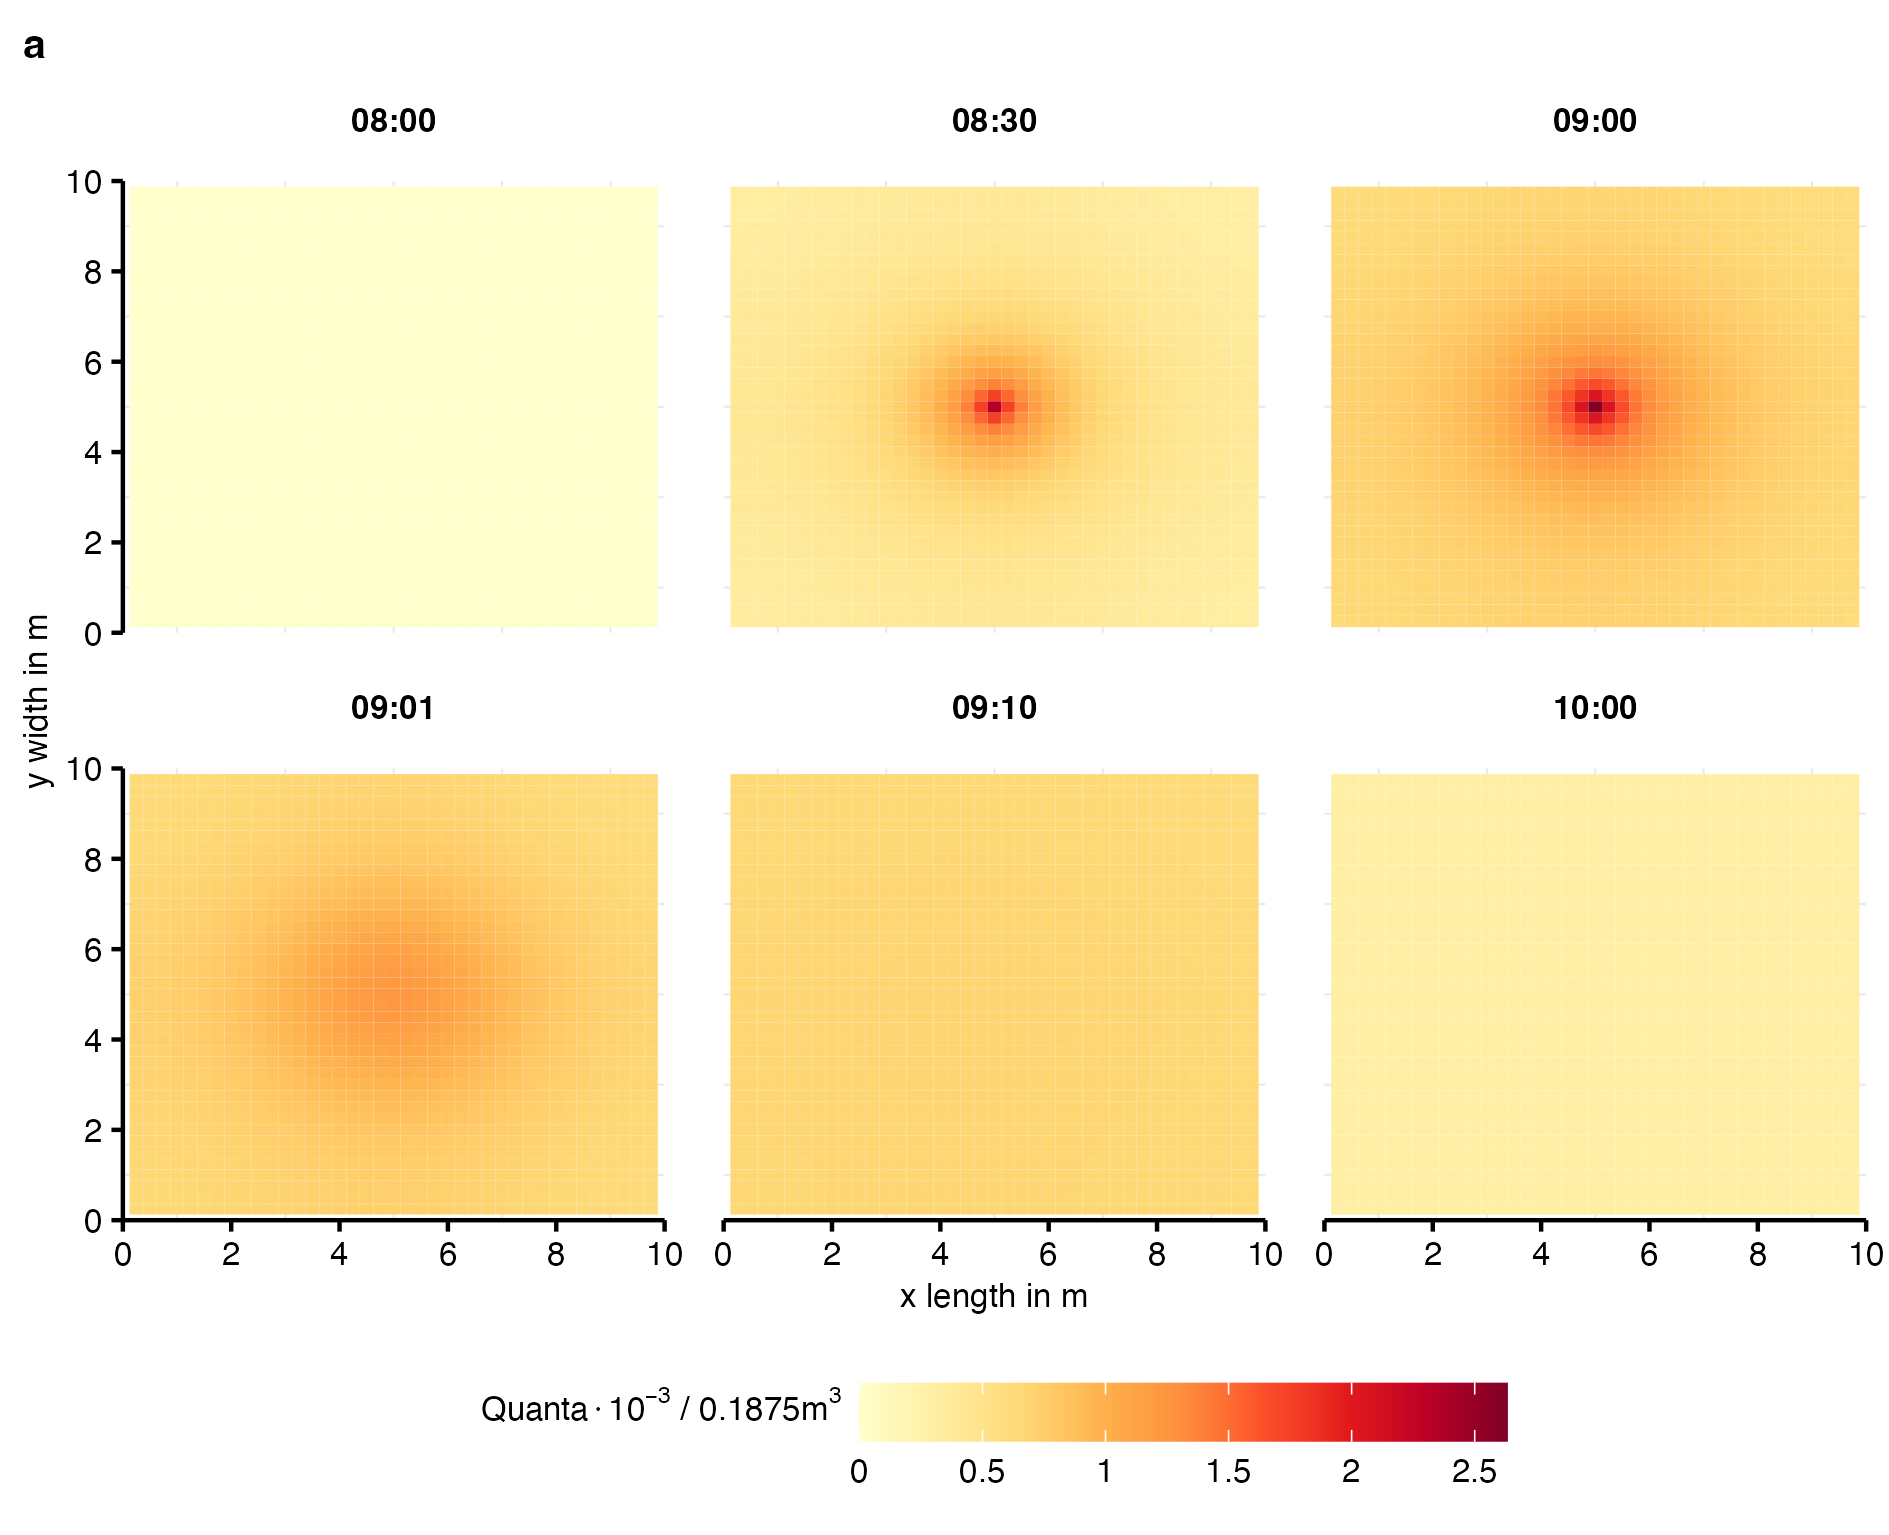
\includegraphics{tests/stm_v2-toy_example.png}
    \caption{Spatiotemporal quanta concentration between 8am and 10am following the generation of quanta by an infectious individual between 8am and 9am in the middle of the room.}
    \label{fig:toy-example}
\end{figure}

\clearpage


\section{Simulation approach}\label{sec:estimation}

\subsection{Setup}\label{prep:building}

We divide the clinic into three spaces: the waiting room (length = 10.55m $\times$ breadth = 5.50m $\times$ height = 3.00m), the corridor (length = 12.45m $\times$ breadth = 2.20m $\times$ height = 2.50m), and the TB room (length = 4.75m $\times$ breadth = 3.50m $\times$ height = 3.00m). We separate the waiting room and the corridor because separate rectangular rooms simplify modeling and because we observe small differences in the time-varying CO$_2$ levels, suggesting these rooms are somewhat different. However, we note that the doors to the corridor were often most of the time, so that the corridor and waiting room were not completely enclosed. As such, it is possible that aerosolized \emph{Mtb} (quanta) spreads from the waiting room to the corridor, and vice versa, but this is not considered in our modeling approach. We rasterize each room into a grid of cubic cells with a squared area of 0.25m$^2$, corresponding to a diagonal length of $\sqrt{0.25^2 + 0.25^2} = 0.35$\,m. Since the rooms have different height, the quanta concentration in the corridors' cells will (all else equal) be higher than in the waiting and TB room by a factor of 3/2.5 = 1.2. 

We model the spatiotemporal quanta concentration during clinic hours from 8am to 4pm and analyze the modeled concentration by daytime, \ie morning (8am to 12am) and afternoon (12am to 4pm). Correspondingly, we estimate the outdoor air exchange rate by daytime, thereby considering potential differences in ventilation patterns between the morning and afternoon. We update the quanta concentration every second at $t = 1, \dots, T$, which aligns with the frequency of the tracking data. We assume that the quanta concentration at $t=0$ is zero anywhere in the airspace, \ie $N_{c,0} = 0 ~~ \forall c$. In other words, we assume that all quanta from the previous day has been removed from the air before the start of the following clinical day. 


\subsection{Monte-Carlo simulation}

We use Monte-Carlo simulation to estimate the risk of infection, thereby considering uncertainty in several modeling parameters. Each simulation consists of the following steps:
\begin{itemize}
    \item[1.] \textbf{Sample uncertain modeling parameters}: Undiagnosed TB patients among clinic attendees, quanta generation rate, the mask reduction rate, and the bacterial inactivation rate.
    \item[2.] \textbf{Compute quanta concentration}: Based on the generation of infectious quanta by diagnosed and undiagnosed TB patients, compute the spatiotemporal quanta concentration in each cell of the rooms over time.
    \item[3.] \textbf{Estimate risk of infection}: Based on their spatiotemporal quanta exposure, estimate the risk of infection for each clinic attendee using the Wells-Riley equation.
\end{itemize}

Most clinic attendees could be undiagnosed TB patients and prior uncertainty in the quanta generation, mask reduction, and bacterial inactivation rate is large. To reflect this uncertainty, we perform 5,000 Monte Carlo simulations and compute the individual risk of infection as the mean or median across these simulations.  

\subsection{Modeling assumptions and prior distributions}\label{sec:priors}

\subsubsection{Initial spread}

We model the amount of quanta that is generated and how it diffuses. What we have not yet discussed is the initial spread of infectious quanta, referred to as the propagation distance, which is the maximum distance from the source to the end of the exhaled air before dispersion. An analysis of exhalation activities suggest a propagation distance of 0.7m\cite{Tang2013PLoSOne}, but larger distances may be reached depending on the activity (\ie breathing, speaking, coughing). Face masks reduce the propagation distance both by blocking (the mask capturing particles) and deflecting (leakage of particles on the sides of the mask) particles\cite{Tang2009RoyalInt,Hui2012PLoSOne,Mansour2013AerosolMed}. Therefore, we assume that mask wearing confines the quanta generation only to the cell where the infectious individual is located. In our setup, this corresponds to a propagation distance of 0.35m (the diagonal cell length) and an area of 0.25$^2$m$^2$. In a hypothetical scenario, we estimate the risk of infection if mask wearing would not have been compulsory. Without masks, we assume double the propagation propagation distance, \ie 0.7m (the diagonal lengths of two cells)\cite{Tang2013PLoSOne}. Since we could not observe the flow direction of the initially generated quanta, we assume that all neighbouring cells are affected equally. That is, we divide the generated quanta equally among the nine affected cells, \ie the cell where the infectious person is located as well as all first-neighbouring cells.


\subsubsection{Quanta generation rate}

Previous studies estimated the quanta generation rate of \emph{Mtb} using the Wells-Riley model\cite{Andrews2014JID,Riley1962ARRD,Escombe2008PLoSMed,Nardell1991ARRD,Dharmadhikari2012AJRCCM}. Andrews et al.\cite{Andrews2014JID} reported an estimate of 0.89\,(quanta h$^{-1}$) (range from 0.44 to 5.69), close to the early estimate provided by Riley et al.\cite{Riley1962ARRD} with 1.25\,quanta h$^{-1}$. On the other end, Escombe et al.\cite{Escombe2008PLoSMed} arrived at an average estimate of 8.2\,quanta h$^{-1}$, which, however, could be as high as 226\,quanta h$^{-1}$. Lower rates were observed in lower for non-multidrug-resistant (MDR), smear-negative patients and considerably higher for MDR, smear-positive TB patients\cite{Escombe2008PLoSMed}. Dharmadhikari et al.\cite{Dharmadhikari2012AJRCCM} also estimated a high average rate of 138\,quanta h$^{-1}$ in MDR TB patients. Nardell et al.\cite{Nardell1991ARRD} also reported a higher estimate of 13\,quanta h$^{-1}$, but only for a single index case. The wide range of estimates within and between studies suggest that the emitted quanta varies considerably with the infectiousness of \emph{Mtb} patients\cite{Wurie2016BMJ}. To consider such variation, Mikszewski et al.\cite{Mikszewski2021GF} used the bacterial load distribution in sputum to estimate the quanta generation rate with the approach developed by Buonanno et al.\cite{Buonanno2020EI}. We have recently adopted this approach to derive quanta generation rate distributions for different activity levels in a school setting\cite{Banholzer2024PGPH}. Here, we follow the same approach to derive a quanta generation rate distribution for sitting and walking activities, assuming 80\% breathing and 20\% speaking during both activities. The resulting prior distributions are shown in \Cref{fig:quanta-distribution}. The quanta generation rate follows a lognormal prior distribution with median 1.08\,quanta h$^{-1}$ (95\%-credible interval [CrI] 0.003\,quanta h$^{-1}$\,$-$\,386\,quanta h$^{-1}$) while sitting and 2.81\,quanta h$^{-1}$ (95\%-CrI 0.008\,quanta h$^{-1}$\,$-$\,987\,quanta h$^{-1}$) while walking. The activity is determined based on whether the distance between two patient tracks was more (walking) or less (sitting) than 0.25m. 

\begin{figure}[!htpb]
    \centering
    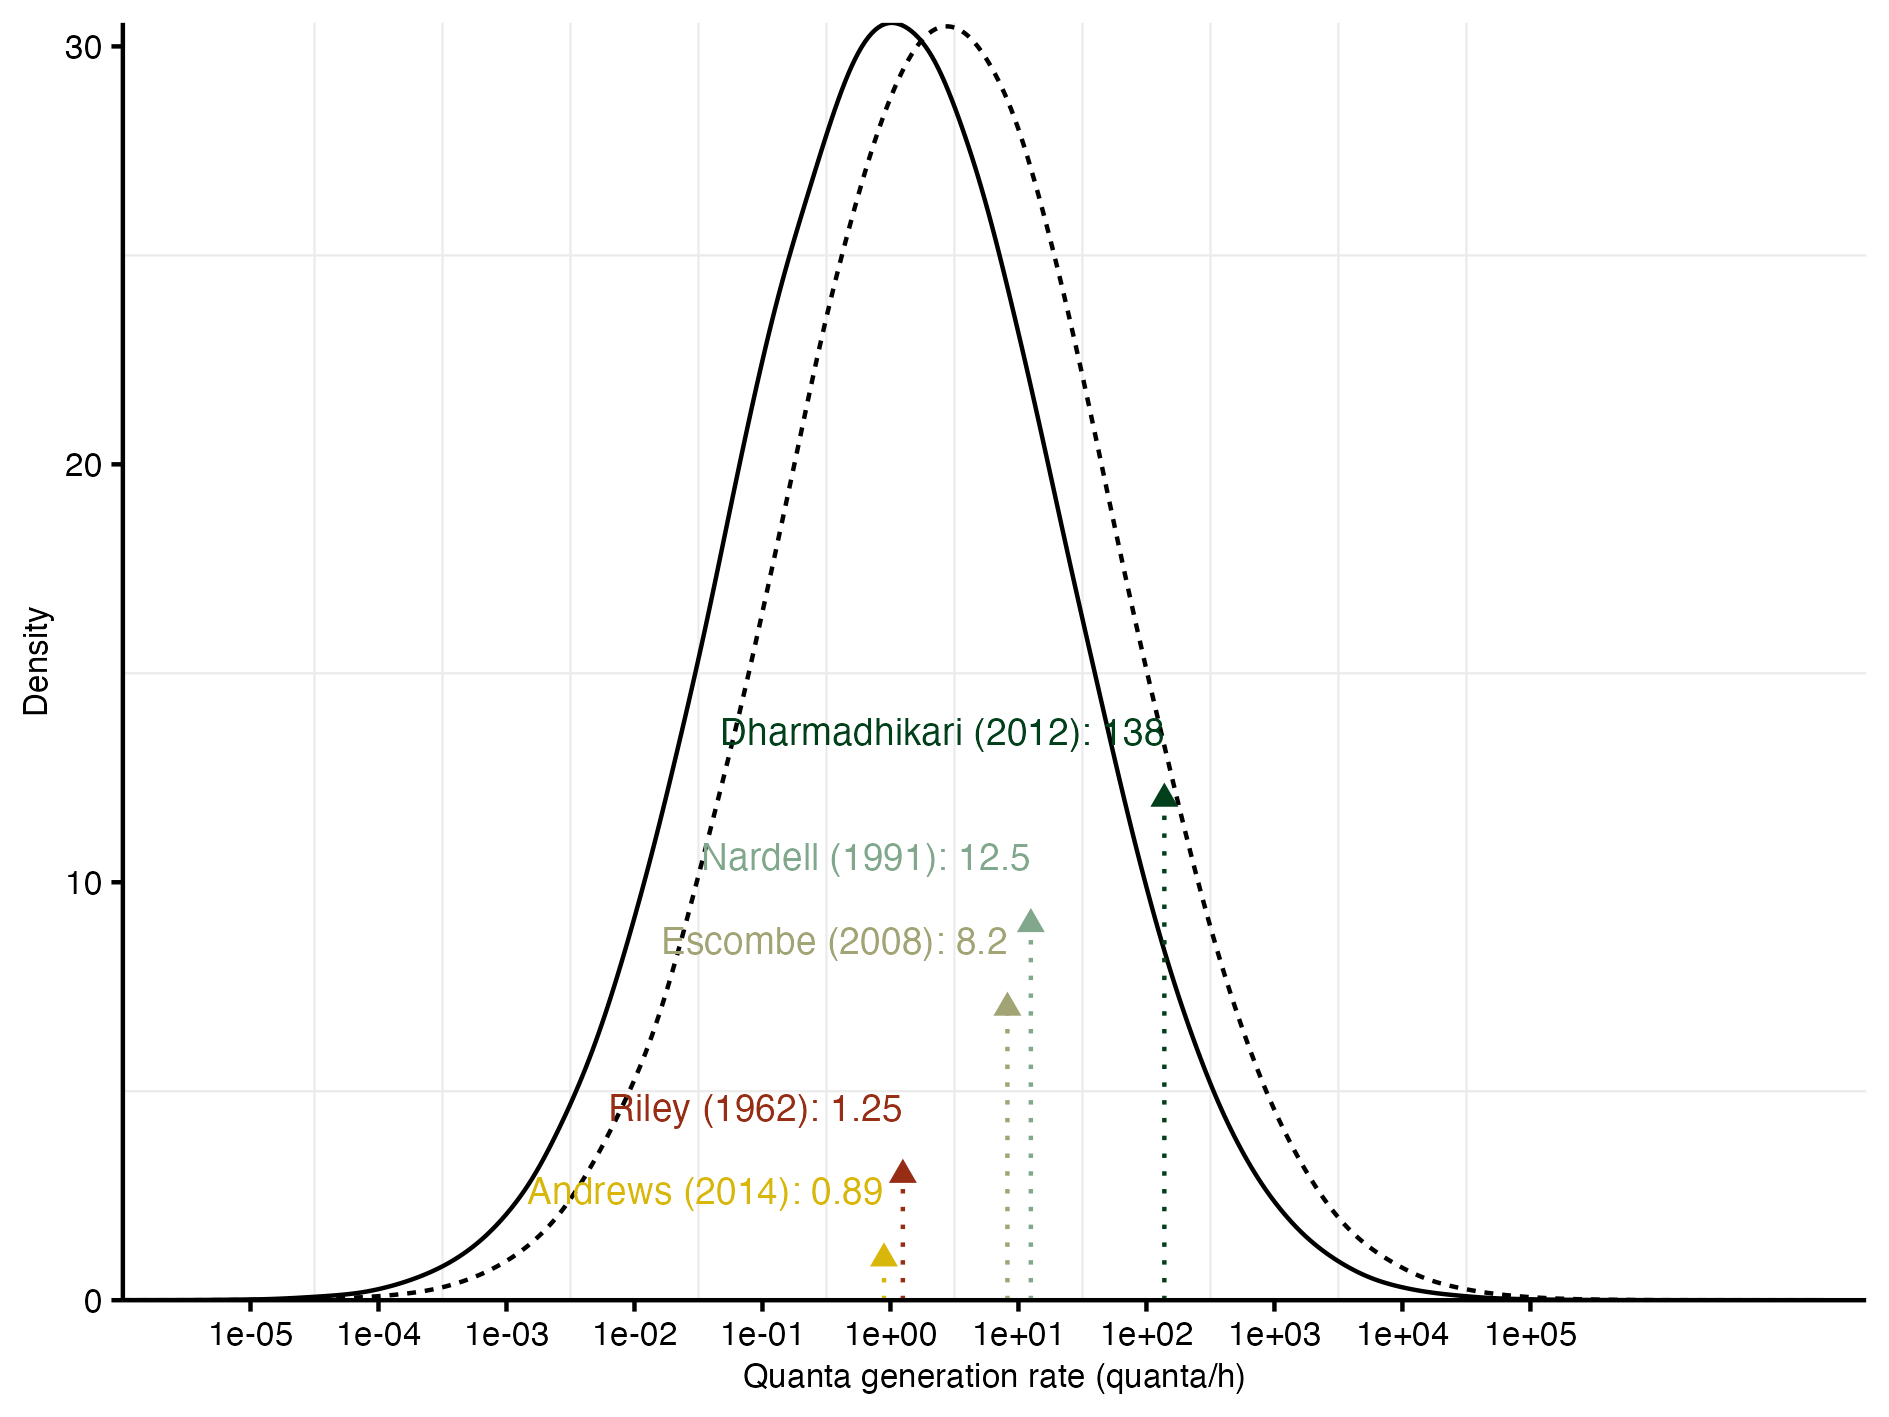
\includegraphics{results/inputs/quanta-generation-rate.png}
    \caption{Prior distribution (log scale) for the quanta generation rate (quanta h$^{-1}$) by activity level (sitting and walking), along with reported average estimates from the literature\cite{Andrews2014JID,Riley1962ARRD,Escombe2008PLoSMed,Nardell1991ARRD,Dharmadhikari2012AJRCCM}.}
    \label{fig:quanta-distribution}
\end{figure}

\subsubsection{Mask reduction rate}

Face masks reduce the number of viral-laden aerosols that are exhaled into the air\cite{Milton2013PLoSPathogens,Leung2020NatMed} and should thus lower the generation of infectious quanta. McCreesh et al. assumed a reduction by masks of 75\% (95\%-confidence interval (56\% to 85\%) based on the findings of Dharmadhikari et al.\cite{Dharmadhikari2012AJRCCM}. Based on that, we model the reduction by masks with $\mathrm{Beta}(24.9, 8.3)$ distribution. We assume that masks were correctly worn the whole time by all clinic attendees and staff during the COVID-19 pandemic. 

\subsubsection{Bacterial inactivation rate}

The bacterial inactivation rate for \emph{Mtb} has not been precisely estimated. Loudon (1969)\cite{Loudon1969AMRRD} report a half-life for aerosolized TB bacilli of 6h ($\lambda$ = 0.12). By contrast, Lever (2000)\cite{Lever2000LettersAppliedMicrobio} reported a half-life of just 5min ($\lambda$ = 8.3). The difference could be explained by differences in humidity levels during the study\cite{Lever2000LettersAppliedMicrobio}: Loudon (1969) studied survival during a relative humidity of about 50\% whereas Lever (2000) studied survival during a relative humidity of about 70\%. Relative humidity in our study is closer to 50\%, thus the estimate by Loudon (1969) seems more representative of the our study conditions.  Moreover, Gannon (2007)\cite{Gannon2007ResVetSci} report a half-life of 1.5 hours ($\lambda$ = 0.46) at relative humidity of over 75\%, yet the estimate is for \emph{Mtb bovis}. In contrast to that, Klein (2014)\cite{Klein2014IJMyco} observe a 80\% reduction within 30min ($\lambda$ = 3.2), which would be closer to Lever (2000). Considering the variation in these estimates, we model $\lambda$ with a $\mathrm{Lognormal}(\mu = \log 1, \sigma = 1)$ distribution, which has a median rate of 1\,quanta h$^{-1}$ (95\%-CrI 0.1\,quanta h$^{-1}$\,$-$\,7.1\,quanta h$^{-1}$). The distribution is shown in \Cref{fig:lambda-distribution} along with the estimates from the literature.

\begin{figure}[!htpb]
    \centering
    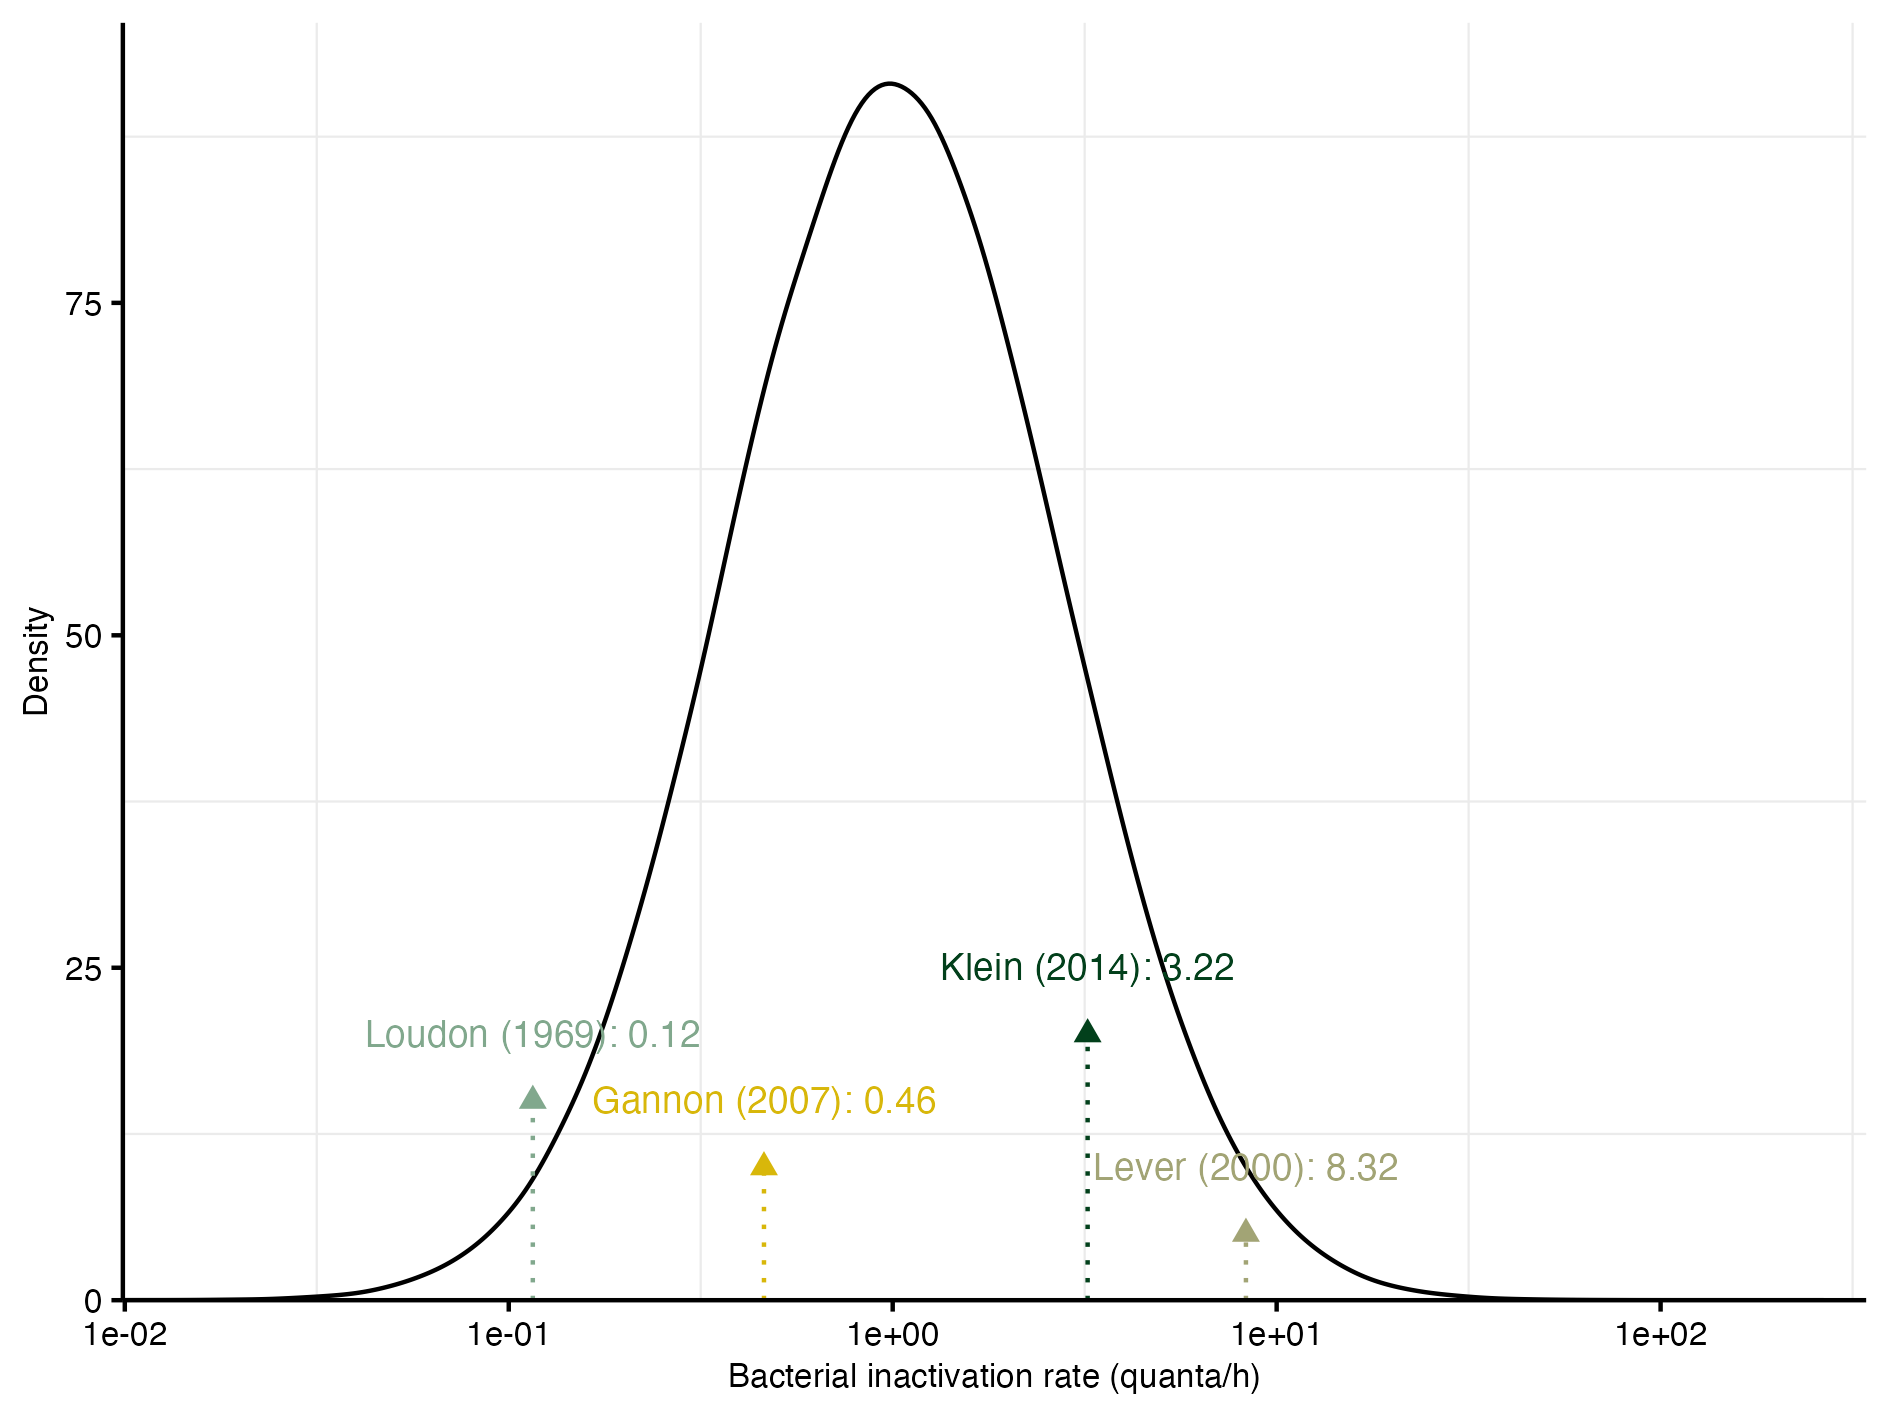
\includegraphics{results/inputs/bacterial-inactivation-rate.png}
    \caption{Prior distribution (log scale) for the bacterial inactivation rate (quanta h$^{-1}$) of \emph{Mtb} along with reported estimates from the literature\cite{Loudon1969AMRRD,Gannon2007ResVetSci,Klein2014IJ,Lever2000LettersAppliedMicrobioMyco}.}
    \label{fig:lambda-distribution}
\end{figure}

\subsubsection{Number of undiagnosed TB patients}

Undiagnosed (subclinical) TB patients may go undetected because they do not show symptoms according to the WHO 4-question symptom screen (cough, fever, weight loss, and night sweats), or the diagnosis could not be made at first presentation based on existing tests\cite{Patterson2023Preprint}. Previous studies suggest that the number of undiagnosed (subclinical) TB patients is roughly similar to the number of diagnosed TB patients\cite{Berhanu2023CID,Moyo2022LancetID}. Therefore, we model the number of undiagnosed TB patients with a Multinomial distribution based on the counts of the daily number of diagnosed TB patients during our study period from October to November 2021 (\Cref{fig:undiagnosed-distribution}. We assume that all clinic attendees can be potential undiagnosed TB patients and sample among them with equal probability. We further assume that undiagnosed and diagnosed TB patients have the same quanta generation rate.

\begin{figure}[!htpb]
    \centering
    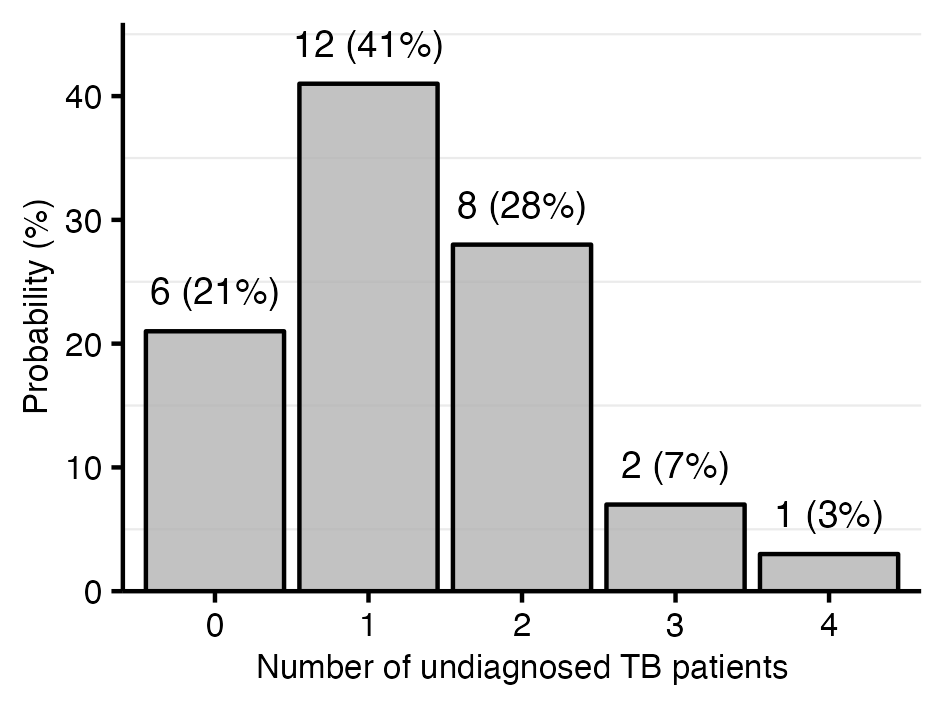
\includegraphics{results/inputs/undiagnosed-tb-patients.png}
    \caption{Counts (\%) of the daily number of diagnosed TB patients visiting the clinic according to clinical records. The number of diagnosed patients is modeled with a Multinomial distribution based on these counts.}
    \label{fig:undiagnosed-distribution}
\end{figure}

\subsubsection{Breathing rate}

Adam et al.\cite{Adams1993} reports breathing (inhalation) rates for different activity levels and by sex. We use the average breathing rate for two activity levels: sitting with $p = 0.51$\,m$^3$ h$^{-1}$ and walking (slowly at 2.5 mph) with $p = 1.33$\,m$^3$ h$^{-1}$. Again, the inhalation rate for each susceptible clinic attendee is determined based on whether the distance between two tracks was more (walking) or less (sitting) than 0.25m. 

\clearpage

\section{Discussion of factors affecting the risk of airborne infection}\label{sec:depth-discussion}


The generation, dispersion, and survival of infectious particles in the air is subject to considerable uncertainty. Therefore, Wells\cite{Wells1955} introduced the concept of a ``quantum'' (infectious dose) to capture the stochastic nature of airborne transmission. A higher concentration of infectious quanta corresponds to a higher probability for an individual to get infected. The probability of infection is modeled with a Poisson relation and the Wells-Riley model considers multiple determinants for the generation and survival of infectious quanta. Nevertheless, transmission events are difficult to predict as the occurrence depends on multiple other factors that can broadly be categorized into (1)~environmental factors, (2)~physicochemical properties of the pathogen, and the (3)~infectiousness of the source and susceptibility of the host. 

\subsection{Environmental factors}

Environmental factors are somewhat considered by our model using CO$_2$ as a tracer gas to estimate quanta diffusion and removal. The combination of clinical and video sensor data further allows the spatial modeling of quanta generation. This makes our approach unique compared to existing modeling based on the Wells-Riley equation assuming a well-mixed airspace\cite{Riley1978AJE,Rudnick2003IndoorAir}. In our spatiotemporal model, we assume a radial diffusion of quanta, which may not reflect the actual airflow at the primary care clinic. The spatial dispersion of infectious particles is often simulated with computational fluid dynamics (CFD) models\cite{Vuorinen2020SafSci,Jung2021InfectChemo,Li2021BuildEnv}. CFD models can simulate a variety of diffusion patterns, which help researchers understanding the influence of airflow. For example, measuring airflow can identify poorly ventilated indoor spaces where infectious particles circulate inside the room rather than getting replaced with fresh outdoor air\cite{Li2021BuildEnv}. However, airflow is rarely considered, especially when it is difficult to assess in a naturally ventilated space, such as our primary care clinic, where the airflow depends on the outdoor wind direction and which doors and windows are open. 

\subsection{Pathogen-specific factors}

Survival and dispersion of aerosols are further determined by the physicochemical properties of virus-laden aerosols such as particle size, viral load, and other chemical components\cite{Wang2021Science}. Currently, these stochastic properties are only indirectly incorporated in the Wells-Riley modeling framework via the quanta generation rate parameter\cite{Riley1978AJE,Rudnick2003IndoorAir}. It is challenging to consider these properties specifically, especially because they can be modified by environmental factors with often unclear, pathogen-specific effects\cite{Songer1967,Chan2011AdvVir,Fernstrom2013JoP,Cox1995Book,Fernstrom2013JoP,Tang2009Interface}. For example, survival of bacteria in aerosols decreases with temperatures $>$24$^{\circ}$C, but the effects of humidity are unclear\cite{Tang2009Interface}. On the one hand, a comparison between two studies suggested that longer airborne survival of \emph{Mtb} could be attributed to lower relative humidity\cite{Loudon1969AMRRD,Lever2000LettersAppliedMicrobio}. On the other hand, airborne \emph{Mtb} was more likely detected in healthcare facilitates with higher relative humidity\cite{Sornboot2019IJTLD,Matuka2021IJERP}.   

\subsection{Patient-specific factors}

Previous studies show considerable variation in the generation of infectious quanta by TB infected patients\cite{Escombe2008PLoSMed,Andrews2014JID}. We model such variation by using a wide prior distribution for the quanta generation rate. Our model could be easily extended to incorporate prior information on the infectiousness of each individual TB patient. In general, only patients with active pulmonary TB are able to produce infectious droplets\cite{Rieder1999}. Infectiousness could be determined based on the most recent sputum test result. Sputum smear positive patients are more likely to transmit \emph{Mtb} than sputum smear negative patients\cite{Shaw1954ART,Brindle1993AMRRD,Grzybowski1975BIUT}. HIV status could further inform both infectiousness and susceptibility. On one hand, HIV-positive patients are more likely to have a negative sputum smear microscopy result than HIV-negative patients, due to the reduced lung cavitation and the fewer \emph{Mtb} bacilli in their sputum\cite{Brindle1993AMRRD,Telzak1997CID}. On the other hand, HIV-positive patients are less prone to control the \emph{Mtb} infection than HIV-negative patients, due to their reduced immune status\cite{Forte1992AIDS,Kwan2011CMR,Shen1988CEI}, and therefore TB disease progresses faster and is often more severe in HIV-positive TB patients compared to HIV-negative patients. 

% data and other limitations
% While we combined multiple data sources to allow spatiotemporal modeling of the generation, spread, and removal of infectious quanta, our data has also limitations. First, clinical attendees could not always be tracked perfectly throughout the clinic using our video sensors. We invested considerable effort to manually link individual tracking IDs probably belonging to the same attendee back together (Supplementary Text~\zref{sec:setting-and-data} in \supp), but some measurement error remains. Second, we linked video tracking and clinical patient data using the times clinical attendees were at the registration and the entry times in the clinical database. False linkages could result when a tracking ID only passed by the registration (without registering) or when multiple IDs were at the registration closely before a clinical entry. Third, to facilitate modeling, we considered the waiting room and corridor as separate, although the door between both rooms was usually open (Supplementary Text~\zref{sec:estimation} in \supp). Fifth, our video sensors could not cover the whole area of the entrance and we did not collect data in the care rooms and other places of the clinic. As a result, the time spent in the clinic and the exposure to infectious quanta may be underestimated for some clinical attendees, although we expect the largest exposure to be in the waiting room, which was fully covered.   


\clearpage

\bibliography{references.bib}

\end{document}